\let\negmedspace\undefined
\let\negthickspace\undefined
\documentclass[journal]{IEEEtran}
\usepackage[a4paper, margin=10mm, onecolumn]{geometry}
%\usepackage{lmodern} % Ensure lmodern is loaded for pdflatex
\usepackage{tfrupee} % Include tfrupee package

\setlength{\headheight}{1cm} % Set the height of the header box
\setlength{\headsep}{0mm}  % Set the distance between the header box and the top of the text

\usepackage{gvv-book}
\usepackage{gvv}
\usepackage{cite}
\usepackage{amsmath,amssymb,amsfonts,amsthm}
\usepackage{algorithmic}
\usepackage{graphicx}
\usepackage{float}
\usepackage{textcomp}
\usepackage{xcolor}
\usepackage{txfonts}
\usepackage{listings}
\usepackage{enumitem}
\usepackage{mathtools}
\usepackage{gensymb}
\usepackage{comment}
\usepackage[breaklinks=true]{hyperref}
\usepackage{tkz-euclide} 
\usepackage{listings}
% \usepackage{gvv}                                        
\def\inputGnumericTable{}                                 
\usepackage[latin1]{inputenc}                                
\usepackage{color}                                            
\usepackage{array}                                            
\usepackage{longtable}                                       
\usepackage{calc}                                             
\usepackage{multirow}                                         
\usepackage{hhline}                                           
\usepackage{ifthen}                                           
\usepackage{lscape}
\usepackage{tikz}
\usetikzlibrary{patterns}

\begin{document}

\bibliographystyle{IEEEtran}
\vspace{3cm}

\title{6.3.3}
\author{ee25btech11063-vejith}

\maketitle
% \maketitle
% \newpage
% \bigskip
{\let\newpage\relax\maketitle}
\renewcommand{\thefigure}{\theenumi}
\renewcommand{\thetable}{\theenumi}
\setlength{\intextsep}{10pt} % Space between text and floats
\textbf{Question}\\
Find the shortest distance between the lines given by\\
$\vec{r} = (8 + 3\lambda) \hat{i} - (9 + 16\lambda) \hat{j} + (10 + 7\lambda) \hat{k}$ and \\$ \vec{r} = 15 \hat{i} + 29 \hat{j} + 5 \hat{k} + \mu (3 \hat{i} + 8 \hat{j} - 5 \hat{k})$\\
\textbf{Solution}:\\
The given lines can be written in vector form as
\begin{align}
    \vec{X}=\myvec{8\\-9\\10}+k\myvec{3\\-16\\7}\\
    \vec{X}=\myvec{15\\29\\5}+k\myvec{3\\8\\-5}\\
    \end{align}
which are of the form
\begin{align}
    \vec{X_1}=\vec{A} + k_1\vec{m_1}\\
    \vec{X_2}=\vec{B} + k_2\vec{m_2}
    \end{align}
     let  $\vec{M}=\brak{\vec{m_1}\hspace{0.5cm}\vec{m_2}}$  and  $\vec{K}=\myvec{k_1\\-k_2}$ be the values of k for which shortest distance between the two lines occurs 

    \begin{align}
    \implies \vec{M}=\begin{pmatrix}
    3 & 3\\
    -16 & 8\\
    7 & -5
        \end{pmatrix} \text{ and }\vec{B-A}=\myvec{7\\38\\-5}\\
         \brak{\vec{M} \hspace{0.5cm} \vec{B-A}}=\begin{pmatrix}
            3 & 3 & 7\\
            -16 & 8 & 38\\
            7 & -5 & -5
        \end{pmatrix}&\xleftrightarrow{R_2 \rightarrow R_2+\frac{16}{3}\times R_1}
        \begin{pmatrix}
            3 & 3 & 7\\
            0 & 24 & \frac{226}{3}\\
            7 & -5 & -5
        \end{pmatrix}\\
        &\xleftrightarrow{R_3 \rightarrow R_3-\frac{7}{3}\times R_1}\begin{pmatrix}
            3 & 3 & 7\\
            0 & 24 & \frac{226}{3}\\
            0 & -12 & -\frac{64}{3}
        \end{pmatrix}\\
        &\xleftrightarrow{R_3 \rightarrow R_3+\frac{1}{2}\times R_2} \begin{pmatrix}
            3 & 3 & 7\\
            0 & 24 & \frac{226}{3}\\
            0 & 0 & -\frac{49}{3}
        \end{pmatrix}
\end{align}
The above matrix now is in row echelon form.Rank of a matix in echelon form is number of non zero rows.so,The rank of the above  matrix is 3\\
$\implies$ given lines are skew.
\begin{align}
\implies \vec{M}^T\vec{M}\vec{K}=\vec{M}^T\brak{\vec{B}-\vec{A}}\\
    \begin{pmatrix}
        3 & -16 & 7\\
        3 & 8 & -5
    \end{pmatrix}\begin{pmatrix}
    3 & 3\\
    -16 & 8\\
    7 & -5
        \end{pmatrix}\vec{K}=\begin{pmatrix}
        3 & -16 & 7\\
        3 & 8 & -5
    \end{pmatrix}\myvec{7\\38\\-5}\\
    \implies \begin{pmatrix}
        314 & -154\\
        -154 & 98
    \end{pmatrix}\vec{K}=\myvec{-622\\350}
\end{align}
The augmented matrix of above equation is given by
\begin{align}
    \left(\begin{array}{cc|c}
        314 & -154 & -622 \\
        -154 & 98 & 350 
\end{array}\right) &\xleftrightarrow{R_1 \rightarrow R_1+ 2R_2} \left(\begin{array}{cc|c}
        6 & 42 & 78 \\
        -154 & 98 & 350 
\end{array}\right)\\ &\xleftrightarrow{R_2 \rightarrow R_2+ \frac{77}{3}\times R_2} \left(\begin{array}{cc|c}
        6 & 42 & 78 \\
        0 & 1176 & 2352 
\end{array}\right)\\
&\xleftrightarrow{R_1 \rightarrow \frac{1}{6}\times R_1} \left(\begin{array}{cc|c}
        1 & 7 & 13 \\
        0 & 1176 & 2352 
\end{array}\right)\\
\text{On back substitution we get, } \\
\vec{K}=\myvec{k_1\\-k_2}=\myvec{-1\\2}
\end{align}

\begin{align}
    \implies \vec{X_1}=\myvec{5\\7\\3} \text{ and }\vec{X_2}=\myvec{9\\13\\15}\\
\end{align}
The minimum distance between the lines is given by
\begin{align}
    \norm{\vec{X_2-X_1}}=\norm{\myvec{4\\6\\12}}=14
\end{align} 
\begin{figure}[h!]
    \centering
    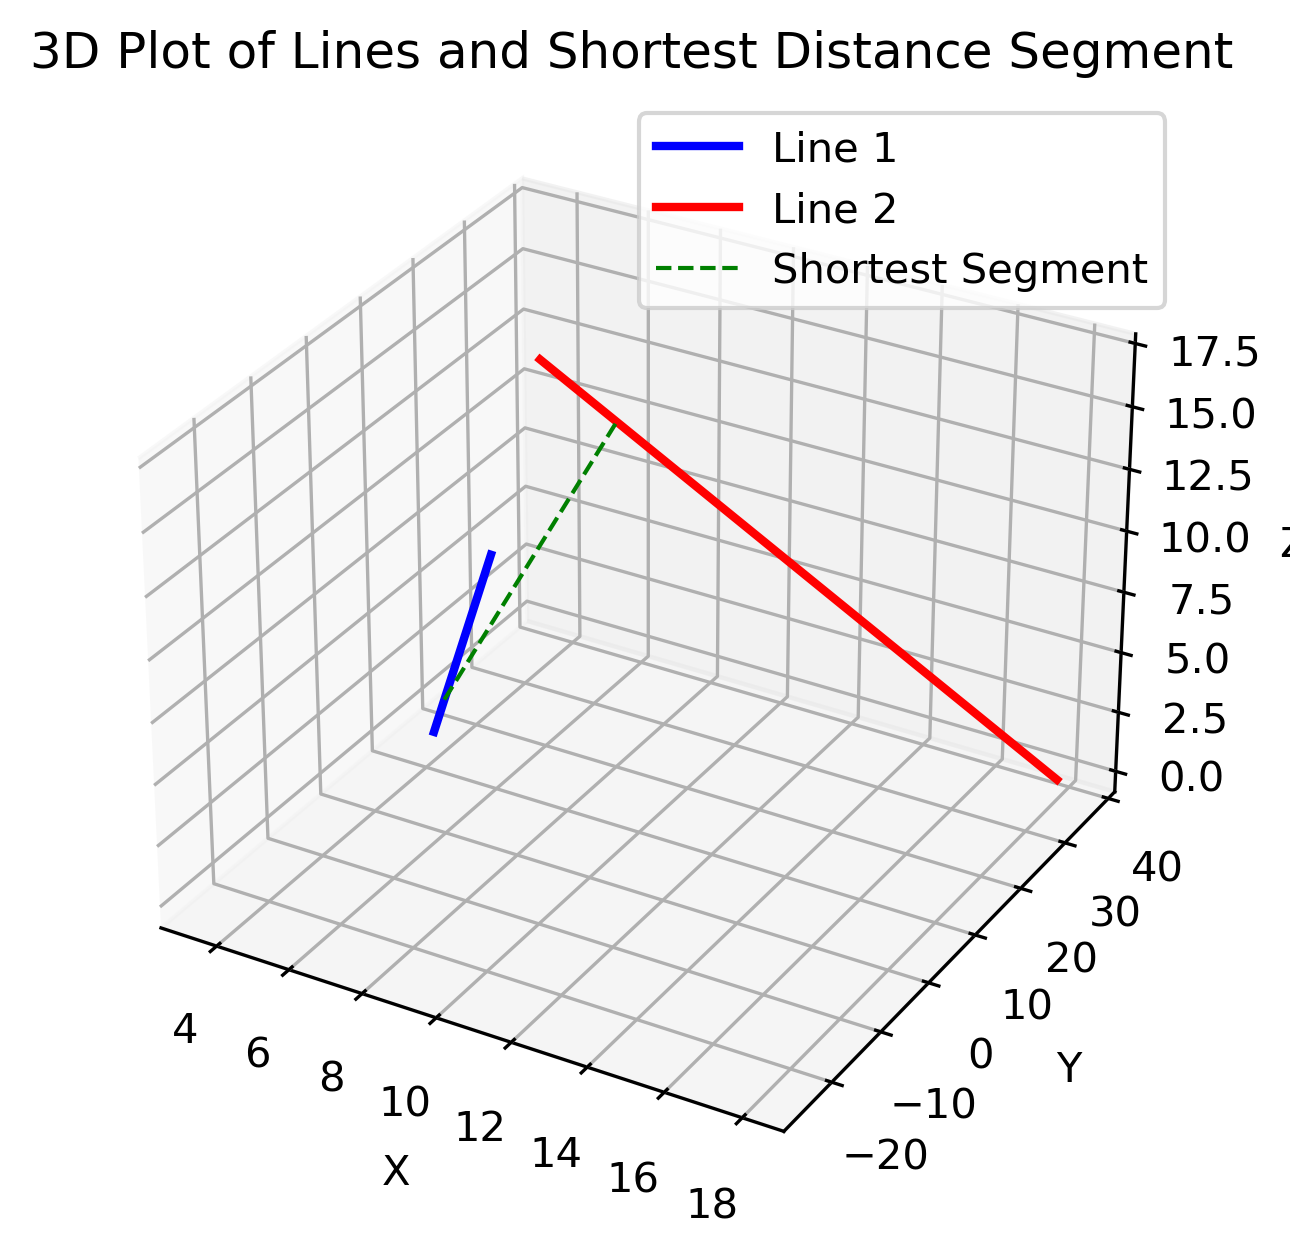
\includegraphics[width=0.5\columnwidth]{figs/01.png}
    \caption{Caption}
    \label{fig:placeholder}
\end{figure}
\end{document}
